\subsection{Ewald selection and mapping to the detector}
\label{sec:correlated_effects}
\label{sec:refraction}
\label{sec:bandwidth_mosaic_cap}
\label{sec:detector_mapping}

The preceding sections introduce four distinct objects that together define the intensity before elastic selection. The structural rod intensity $S_{hk}(L,\lambda_s)$ is a scalar intensity density along the crystallite-frame rod containing the crystallographic amplitude. The location map $\mathbf Q_{hk}(\alpha,\beta,L)$ assigns each rod coordinate and crystallite orientation a point in three-dimensional reciprocal space. The orientation weight $p_m(\alpha,\beta)$ gives the probability density of that crystallite orientation and multiplies the rod intensity. The reciprocal-volume Jacobian $J_{\mathrm{vol},hk}$ converts the weighted measure in $(\alpha,\beta,L)$ coordinates into a physical density per reciprocal-space volume. The selected intensity is then mapped to a 2D area detector.

For one source state $s$, a small pre-Ewald parameter element therefore carries
\begin{equation}
  dI^{\mathrm{pre}}_{hk,s}
  =S_{hk}(L,\lambda_s)p_m(\alpha,\beta)
   \,d\alpha\,d\beta\,dL
  \quad\text{at}\quad
  \mathbf Q_{hk}(\alpha,\beta,L).
  \label{eq:pre_ewald_measure_main}
\end{equation}
The location map changes the associated volume element according to
\begin{equation}
  d^3Q
  =J_{\mathrm{vol},hk}\,d\alpha\,d\beta\,dL,
  \qquad
  J_{\mathrm{vol},hk}
  =\left|\det\frac{\partial\mathbf Q_{hk}}
  {\partial(\alpha,\beta,L)}\right|.
  \label{eq:reciprocal_volume_measure_main}
\end{equation}
Consequently, the reciprocal-space intensity density is the sum of the weighted rod contributions divided by $J_{\mathrm{vol},hk}$. In compact form,
\begin{equation}
  \rho_{Q,s}(\mathbf Q)
  =\sum_{\substack{(h,k),j\\
  \mathbf Q_{hk}(\alpha_j,\beta_j,L_j)=\mathbf Q}}
  \frac{S_{hk}(L_j,\lambda_s)
  p_m(\alpha_j,\beta_j)}{J_{\mathrm{vol},hk,j}}.
  \label{eq:pre_ewald_reciprocal_density_main}
\end{equation}
$S_{hk}$ supplies the structural intensity, $\mathbf Q_{hk}$ supplies its location, $p_m$ supplies its statistical weight, and $J_{\mathrm{vol},hk}$ preserves that intensity under the coordinate transformation.

After the incident optical boundary condition is applied, let $\mathbf k'_{i,s}$ be the internal incident wavevector for source state $s$, with $K_s=|\mathbf k'_{i,s}|$. Before elastic selection, the three coordinates $(\alpha,\beta,L)$ are independent: $\alpha$ and $\beta$ set the crystallite orientation, while $L$ sets the position along the rod. For a fixed source state, rod, and Ewald-intersection branch $j$, the Ewald condition supplies one scalar equation. Solving that equation removes one unknown by determining the compatible intrinsic rod coordinate $L=L_{hk,j,s}(\alpha,\beta)$:
\begin{equation}
  \left|\mathbf k'_{i,s}+\mathbf Q_{hk}(\alpha,\beta,L)\right|=K_s,
  \qquad
  \mathbf Q^{E}_{hk,j,s}(\alpha,\beta)
  =\mathbf Q_{hk}\!\left[\alpha,\beta,L_{hk,j,s}(\alpha,\beta)\right].
  \label{eq:ewald_surface_parameterization_main}
\end{equation}
The Ewald restriction therefore reduces the three-coordinate reciprocal-space description to a two-coordinate surface chart: $L$ becomes the dependent coordinate selected by elasticity, and $(\alpha,\beta)$ remain as the two independent parameters of a local Ewald-surface patch embedded in three-dimensional reciprocal space.

The intensity decorating that patch is obtained by evaluating the rod intensity at the selected $L$ and weighting it by the crystallite-orientation density, the population of the individual $(h,k)$ rod, and the source-dependent optical factors. Schematically,
\begin{equation}
  \rho^{E}_{hk,j,s}(\alpha,\beta)
  \propto
  \frac{p_m(\alpha,\beta)\,
  S_{hk}\!\left[L_{hk,j,s}(\alpha,\beta),\lambda_s\right]W_{hk,j,s}}
  {J_{\mathrm{vol},hk}}.
  \label{eq:ewald_surface_density_main}
\end{equation}
Here $\rho^{E}$ is intensity per unit Ewald-surface area.

Each selected momentum transfer defines the internal exit vector $\mathbf k'_{f,s}=\mathbf k'_{i,s}+\mathbf Q^{E}$. The exit boundary condition converts this vector to the outgoing wavevector in air, and the calibrated detector geometry maps that ray to continuous detector coordinates. This final coordinate change introduces the detector Jacobian $J_{\mathrm{det},s}$, which converts intensity per Ewald-surface area into intensity per detector area. So $J_{\mathrm{vol},hk}$ first establishes the reciprocal-space density, and $J_{\mathrm{det},s}$ then maps the selected surface density to the detector. Their net geometric contribution is $J_{\mathrm{det},s}/J_{\mathrm{vol},hk}$. The detector Jacobian contains the pixel solid angle, detector pose and distance, and the angular area change associated with exit refraction, so no additional solid-angle correction is applied.

Figure~\ref{fig:ewald_to_detector_mapping} visualizes this source-resolved sequence for the nominal Bi$_2$Se$_3$ incidence angle of $5^\circ$. The color on the internal-film Ewald sphere represents the physical intensity per unit Ewald-surface area. The planar and tilted-detector panels show the corresponding detector-coordinate density after the detector Jacobian is applied.

\begin{figure}[H]
  \centering
  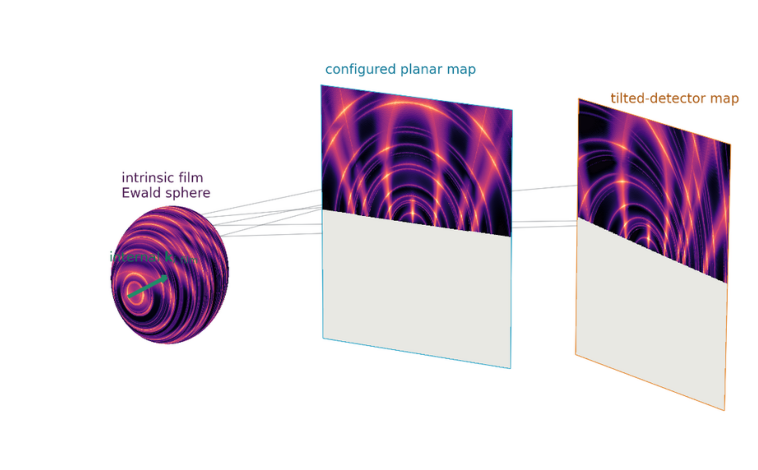
\includegraphics[width=0.68\linewidth]{figures/geometry/ewald_intensity_to_detector_mapping.png}
  \caption{Source-resolved mapping from reciprocal-space intensity to detector coordinates for the nominal Bi$_2$Se$_3$ incidence angle of $5^\circ$. The left panel shows intensity per unit area on the internal-film Ewald surface after the rod, powder-cylinder, mosaic, and reciprocal-volume transformations. The center and right panels show the same selected intensity in the configured planar representation and on the tilted detector after exit refraction and the detector-coordinate Jacobian.}
  \label{fig:ewald_to_detector_mapping}
\end{figure}
\enlargethispage{\baselineskip}

The calculation is repeated independently for every incident state, and the detector densities are summed with their source weights. The resulting image is in the same measurement space as the experimental detector image, so measured and calculated intensities are integrated over identical finite detector regions. Coordinates such as $2\theta$, $\phi$, $Q_R$, and $Q_z$ are downstream representations of this detector intensity. Here $Q_z$ is the momentum-transfer component along the mean film normal and $c$ is the crystallographic repeat length along that direction. The detector-derived projected coordinate used below is
\begin{equation}
  L_{\mathrm{proj}}=\frac{Q_zc}{2\pi}.
  \label{eq:lproj_detector_mapping}
\end{equation}
The crystallite-frame coordinate $L$ identifies where $S_{hk}(L,\lambda_s)$ is evaluated. The projected coordinate $L_{\mathrm{proj}}$ is formed only after orientation, Ewald selection, and detector mapping. The two coincide only in the ideally aligned limit.

\subsection{Reflectivity}
\label{sec:reflectivity}

The motivation for a separate specular treatment is visible directly in Fig.~\ref{fig:hk0_low_l_star}. In addition to the $003$ and $006$ diffraction features, the measured $r=0$ profile contains a much brighter near-origin feature in the near-critical region. Its position and intensity scale identify a specular optical response rather than another finite-stack Bragg peak or independent evidence for a broad mosaic tail.

We therefore describe the measured $r=0$ profile with two limiting calculations. In the near-critical, low-$Q_z$ region, a Parratt recursion accounts for refraction, absorption, evanescence, and multiple reflections at the interfaces.\cite{Parratt1954} Interfacial roughness modifies the Fresnel amplitudes within that Parratt branch through the N\'evot--Croce factor.\cite{NevotCroce1980} At higher $Q_z$, including the $003$ Bragg region, the finite-stack kinematic rod intensity is used. The two branches are placed on the same detector-derived coordinate, background treatment, and intensity scale and are matched smoothly over a declared overlap interval. This practical stitching is the Parratt-to-kinematic crossover.

This construction is used here to keep the near-origin reflectivity distinct from the radial wavelength effect and transverse mosaicity. It is not an independent reflectivity refinement of density, optical constants, roughness, or thickness. Figure~\ref{fig:specular_joint_fit_placeholder} illustrates the intended common-scale comparison. Direct measured and calculated arrays are required before it is used as quantitative evidence.

\begin{figure}[H]
  \centering
  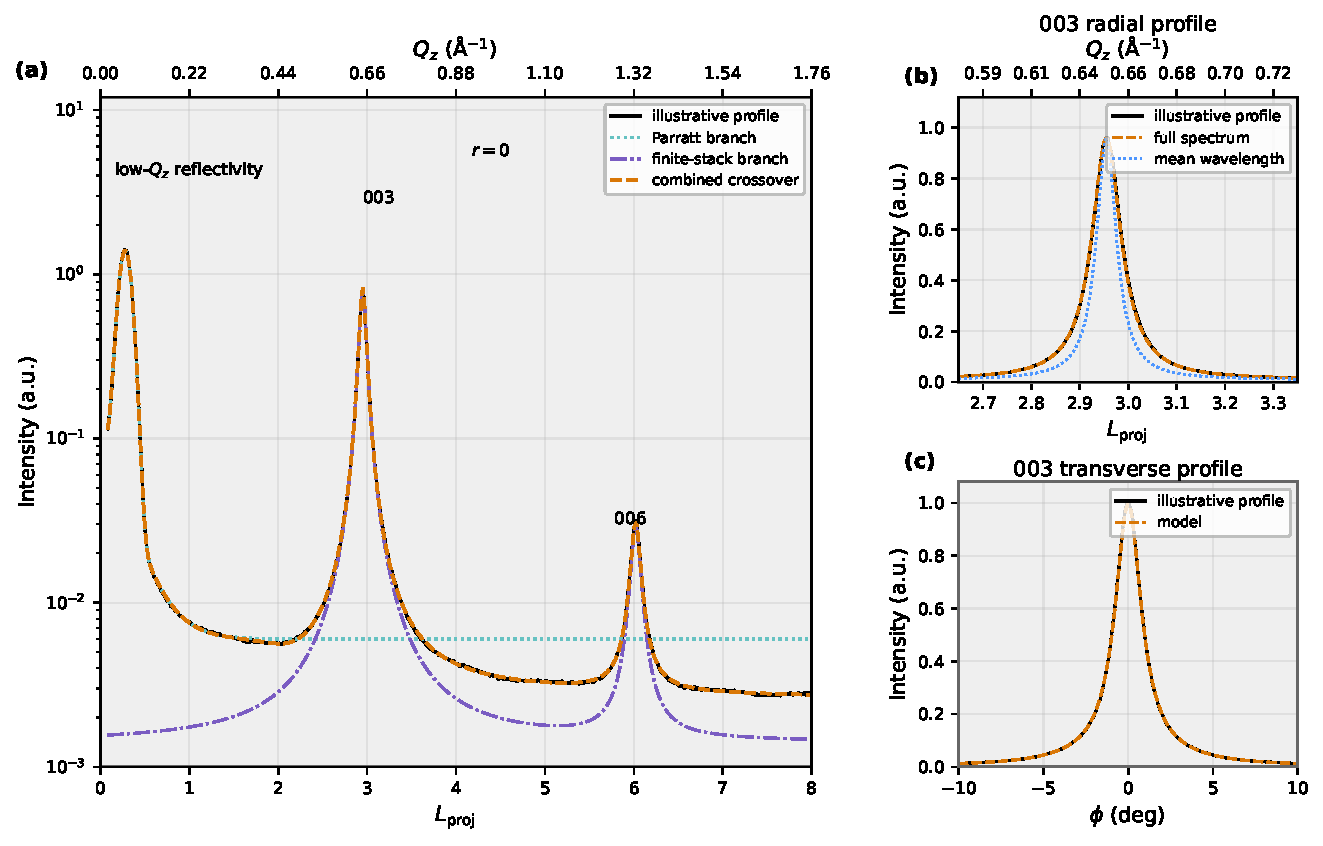
\includegraphics[width=\linewidth]{figures/correlated_effects/fig_specular_parratt_kinematic_003_joint_fit.pdf}
  \caption{Illustrative construction of the stitched $r=0$ specular response from the low-$Q_z$ reflectivity region through the $003$ Bragg peak. (a) The Parratt optical branch, finite-stack kinematic branch, and their smooth Parratt-to-kinematic crossover are shown on one coordinate transformation, background treatment, and intensity scale. N\'evot--Croce roughness is part of the Parratt branch rather than a separate contribution. (b) Expanded radial $003$ profile illustrating the full wavelength-resolved calculation and a mean-wavelength control. (c) Transverse $\phi$ profile illustrating the mosaicity-sensitive direction. The lower horizontal axes use $L_{\mathrm{proj}}$ and the upper axes use $Q_z$. Direct measured and calculated arrays are required before this figure is used as quantitative evidence.}
  \label{fig:specular_joint_fit_placeholder}
\end{figure}
